\subsection{Calibration}
\label{ref:calibration}

It is unfortunate but neccessary that for this method of vehicle classification that for each different location and camera angle an element of calibration is required to obtain best results. This is a function of the size of vehicles in the camera frame and the lighting conditions at the location. Presently these factors are compensated for by manually calibrating the morphological operations and areas of interest for counting and speed measurement. 

\subsubsection{Calibrating Morphological Operations}

To find the optimal morphological structuring element shape and size, and the number of iterations of closing and dilation to perform for the setting in Figure \ref{fig:original_frame} a visual analysis of the effect of a number of settings was performed. For example Figure \ref{fig:morph_testing} show the result of a morphological closure to the output of the background subtractor using different structuring element shapes and closure iterations. 7x7 was formerly settled on as the structuring element size for it produced not too much nor too little effect on the foreground objects. In the visual analysis you seek the result that has converted the most fractured vehicle masks into a single closed contour wit the least iteration, hence for this particular example the optimal morphological closure parameters were a rectangular structuring element with 3 iterations. In Figure \ref{fig:compare_closure} the highlighted shapes have found closure and so will be counted as a single entity in the contouring process.


\begin{figure}[htbp]
    \centering
    \begin{subfigure}[b]{0.42\textwidth}
        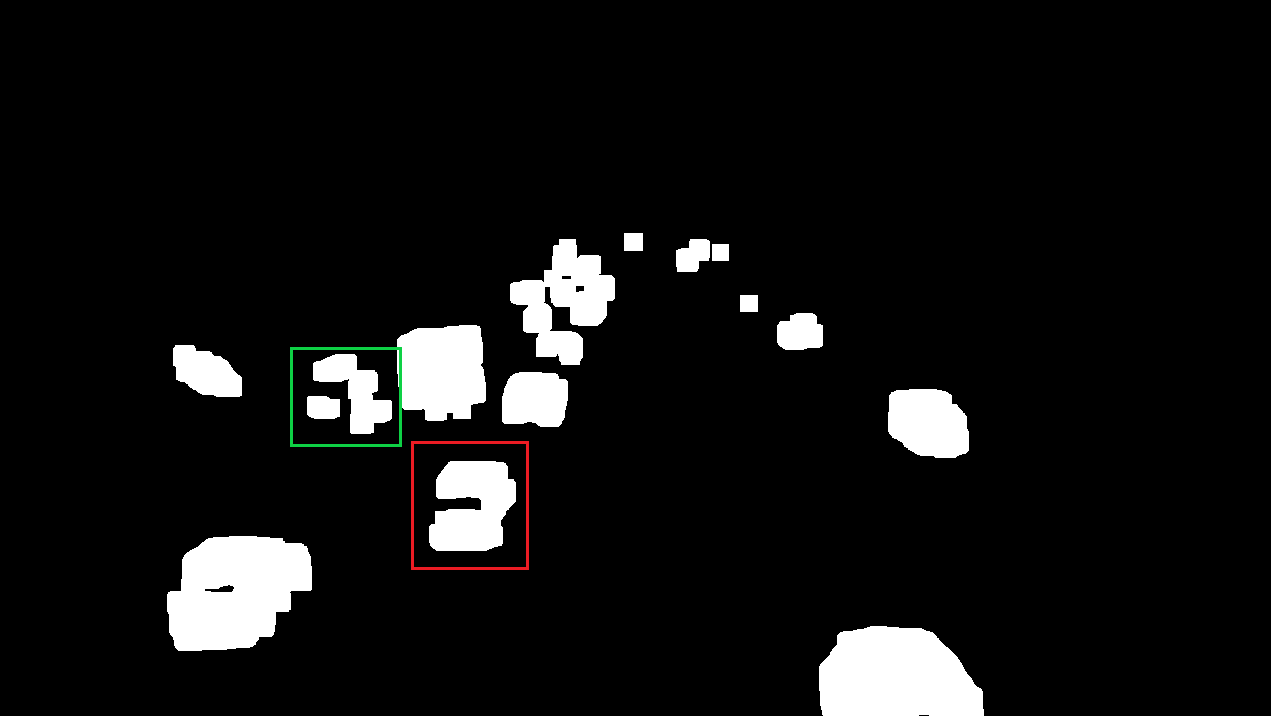
\includegraphics[width=\textwidth]{design/detection/calibration/rect_3_edit}
        \captionsetup{format = hang}
        \caption{Rectangular structuring element closure}
    \end{subfigure}
    \begin{subfigure}[b]{0.42\textwidth}
        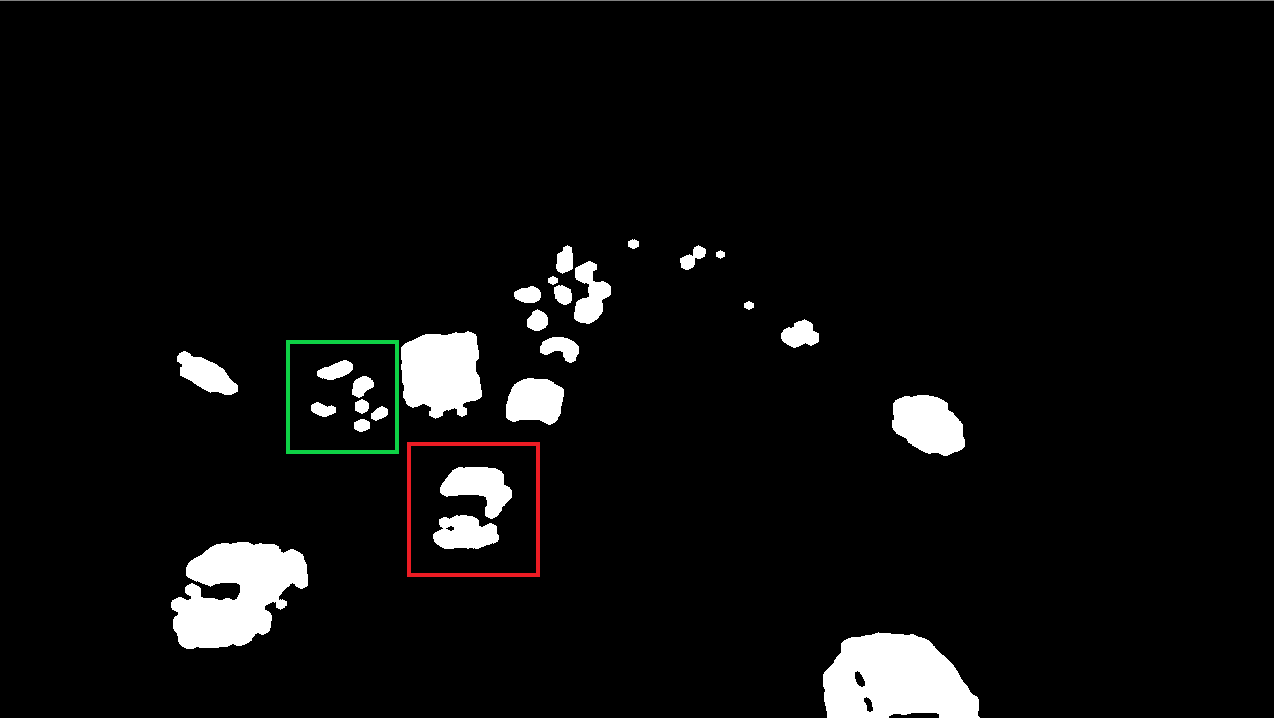
\includegraphics[width=\textwidth]{design/detection/calibration/ellipse_3_edit}
        \captionsetup{format = hang}
        \caption{Elliptical structuring element closure}
    \end{subfigure}
    \captionsetup{format = hang}
    \caption{Comparison of morphological closure using a 7x7 rectangular and elliptical structuring element for 3 iterations.}
    \label{fig:compare_closure}
\end{figure}


\begin{figure*}[htbp]
    \begin{tabular}{
        >{\centering\arraybackslash}m{0.4cm}
        >{\centering\arraybackslash}m{4.5cm}
        >{\centering\arraybackslash}m{4.5cm}
        >{\centering\arraybackslash}m{4.5cm}}
          & Ellipse & Cross & Rectangle \\
        1 
        &
        \begin{subfigure}[b]{0.3\textwidth}
            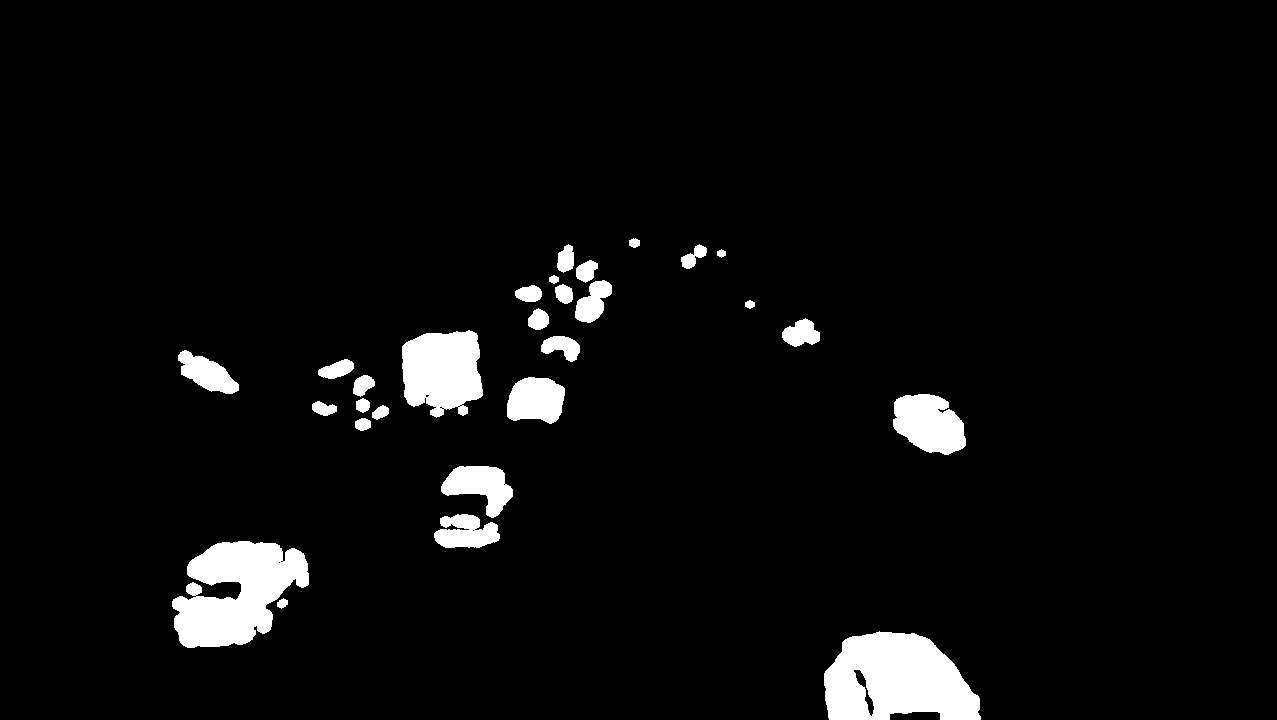
\includegraphics[width=\textwidth]{design/detection/morphology/ellipse_1}
            % \captionsetup{format = hang}
        \end{subfigure} &
        \begin{subfigure}[b]{0.3\textwidth}
            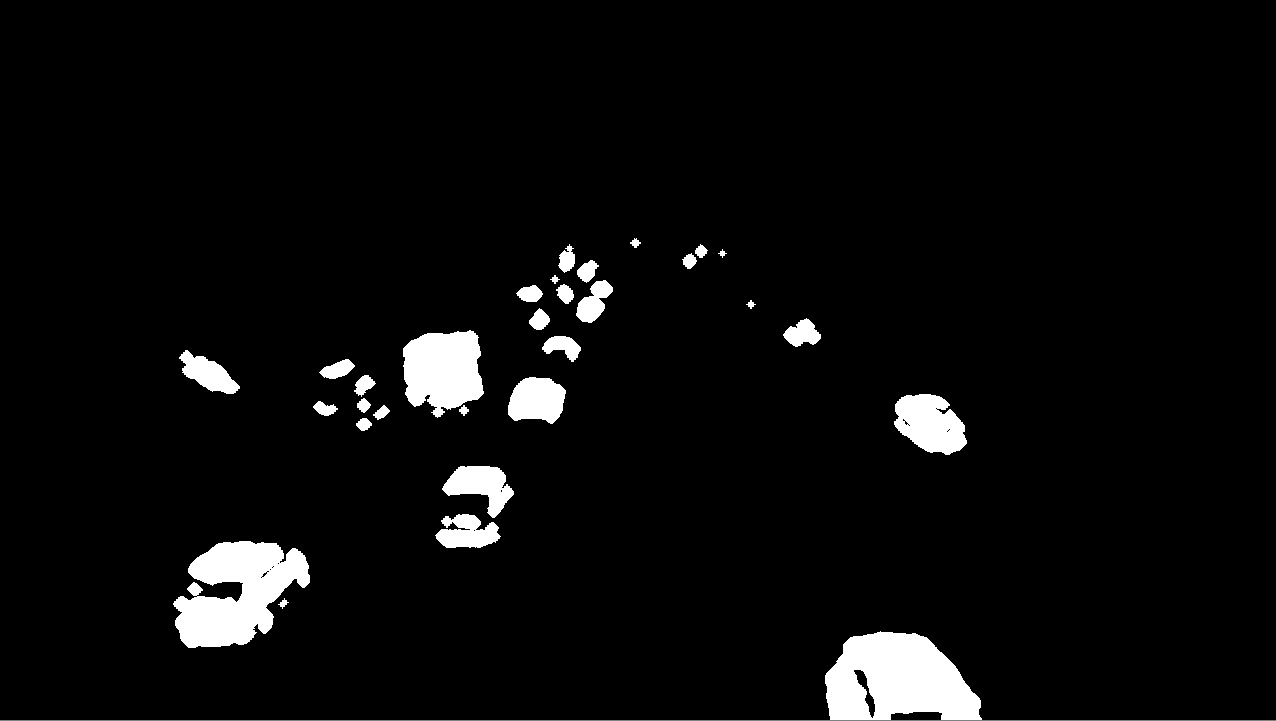
\includegraphics[width=\textwidth]{design/detection/morphology/cross_1}
            % \captionsetup{format = hang}
        \end{subfigure} &
        \begin{subfigure}[b]{0.3\textwidth}
            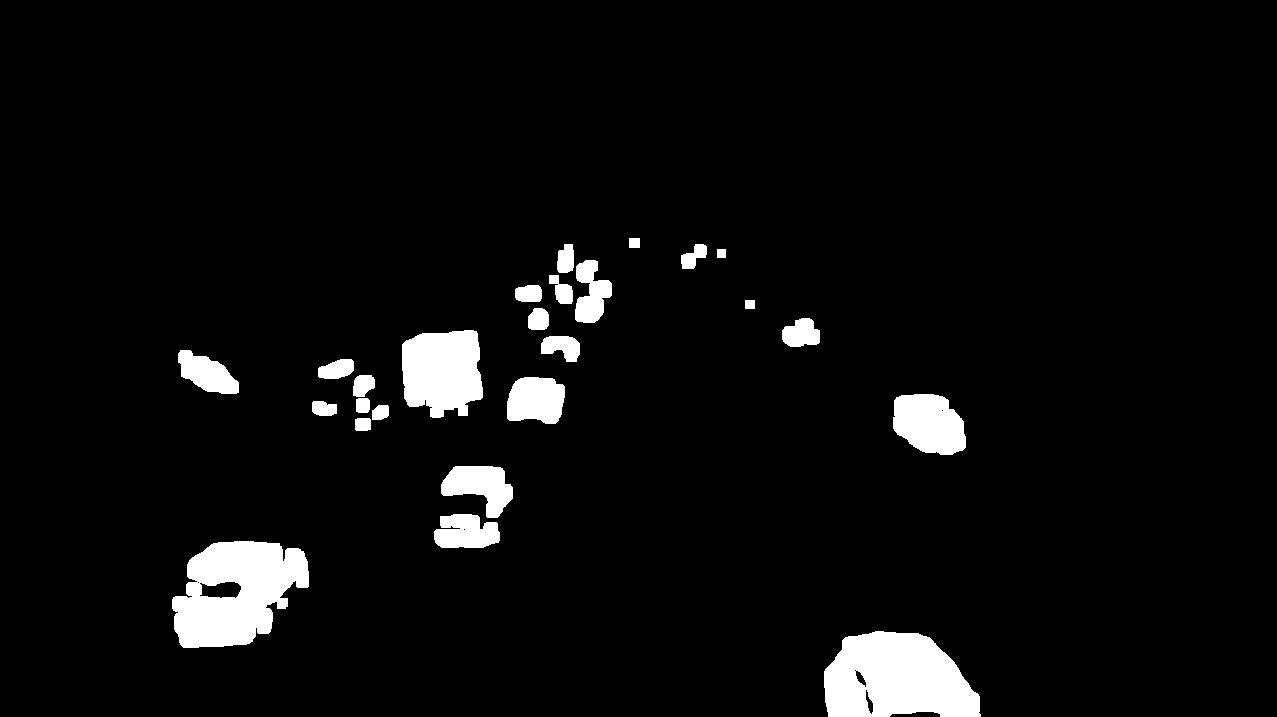
\includegraphics[width=\textwidth]{design/detection/morphology/rect_1}
            % \captionsetup{format = hang}
        \end{subfigure} \\
        3 &
        \begin{subfigure}[b]{0.3\textwidth}
            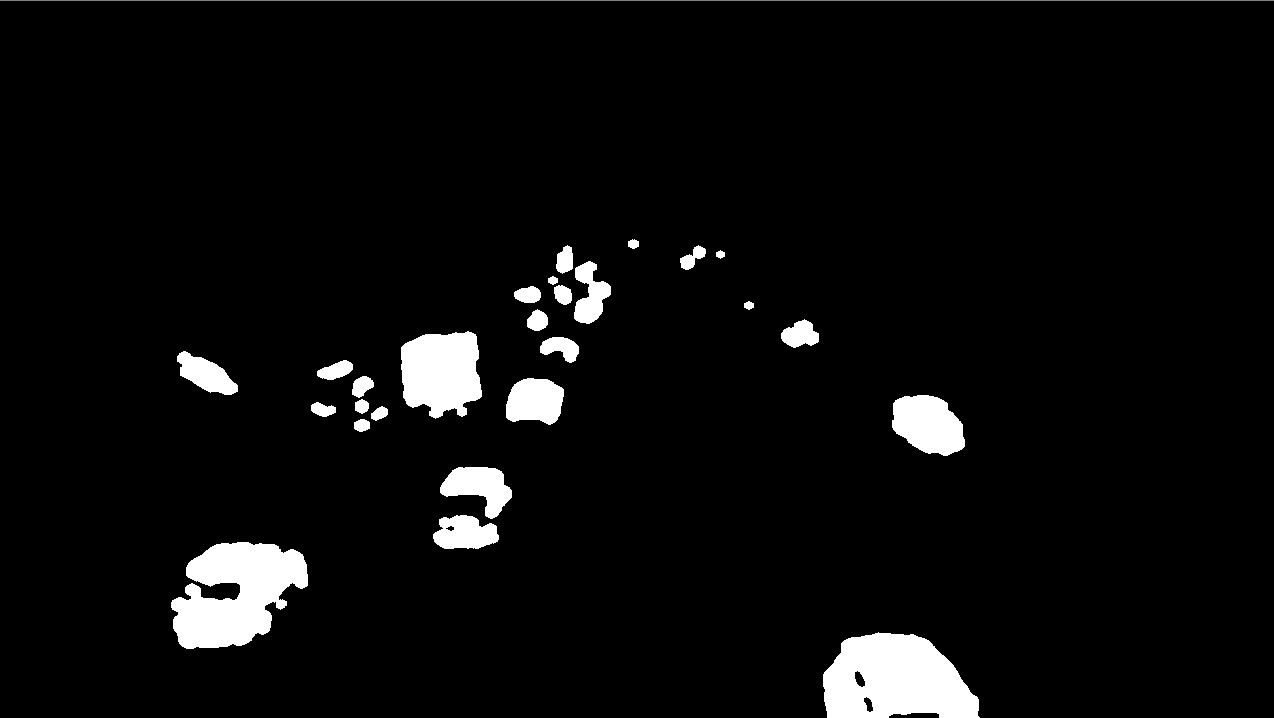
\includegraphics[width=\textwidth]{design/detection/morphology/ellipse_3}
            % \captionsetup{format = hang}
        \end{subfigure} &
        \begin{subfigure}[b]{0.3\textwidth}
            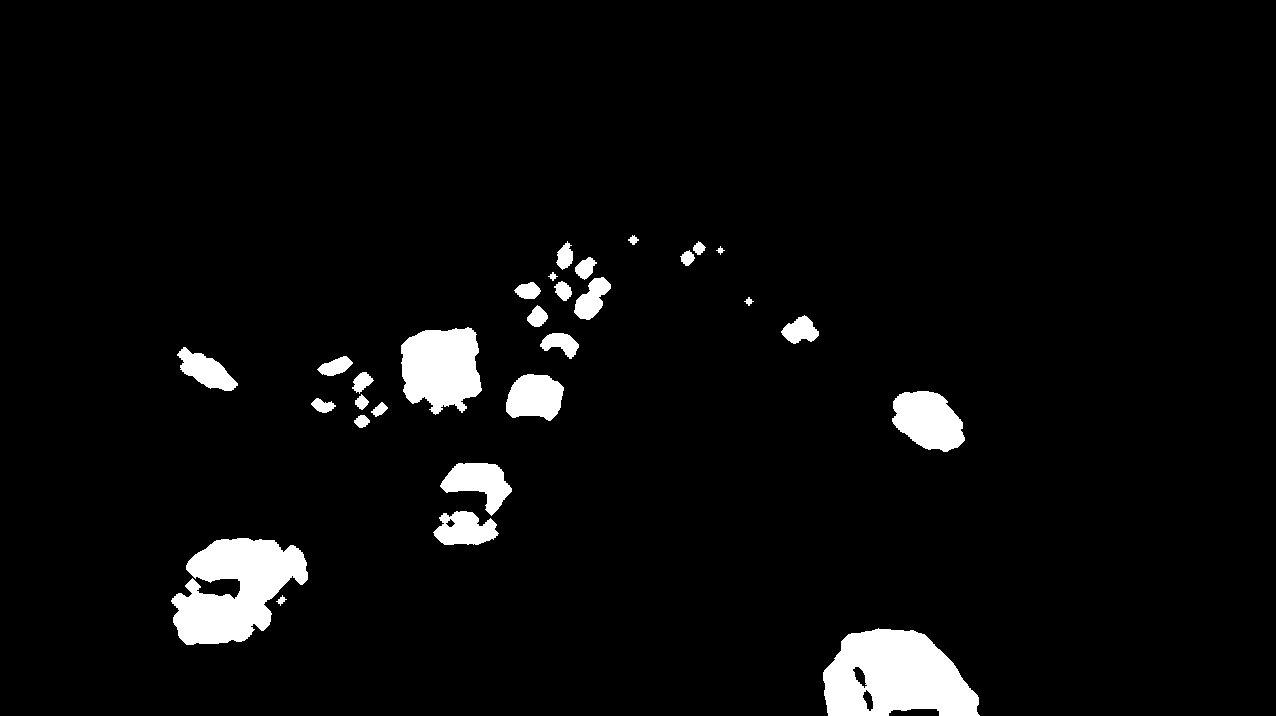
\includegraphics[width=\textwidth]{design/detection/morphology/cross_3}
            % \captionsetup{format = hang}
        \end{subfigure} &
        \begin{subfigure}[b]{0.3\textwidth}
            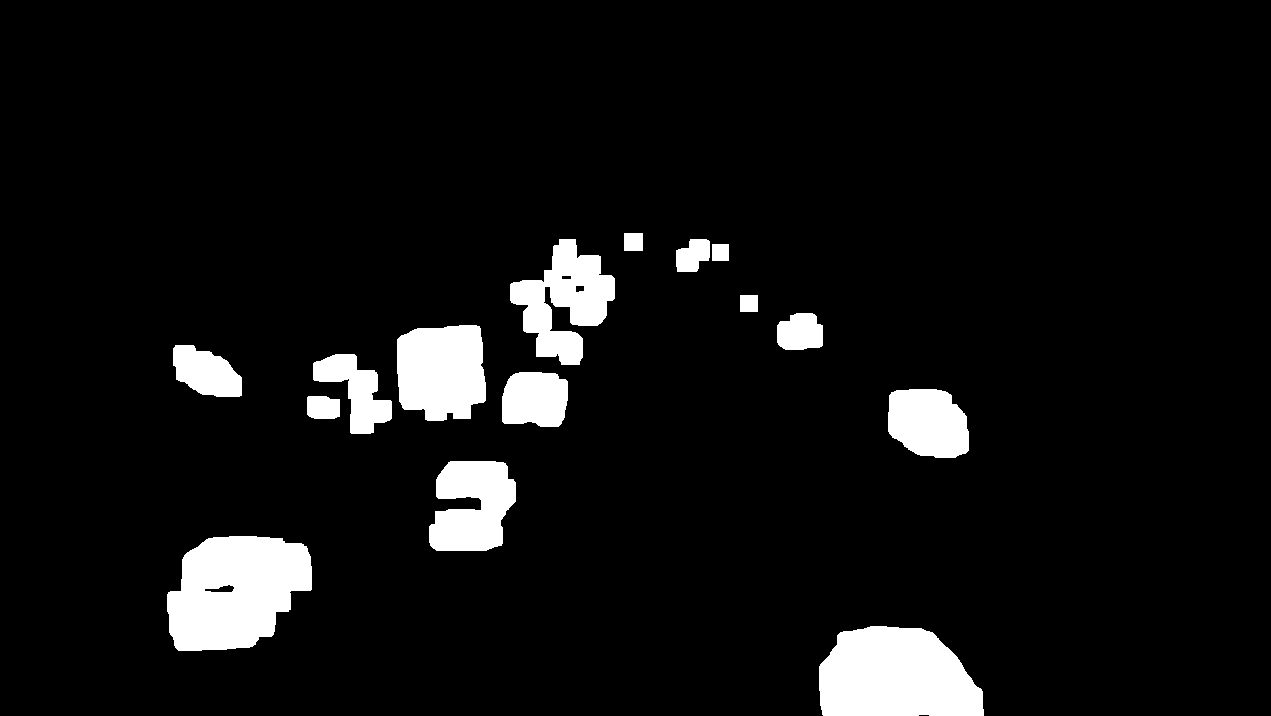
\includegraphics[width=\textwidth]{design/detection/morphology/rect_3}
            % \captionsetup{format = hang}
        \end{subfigure} \\
        5 &
        \begin{subfigure}[b]{0.3\textwidth}
            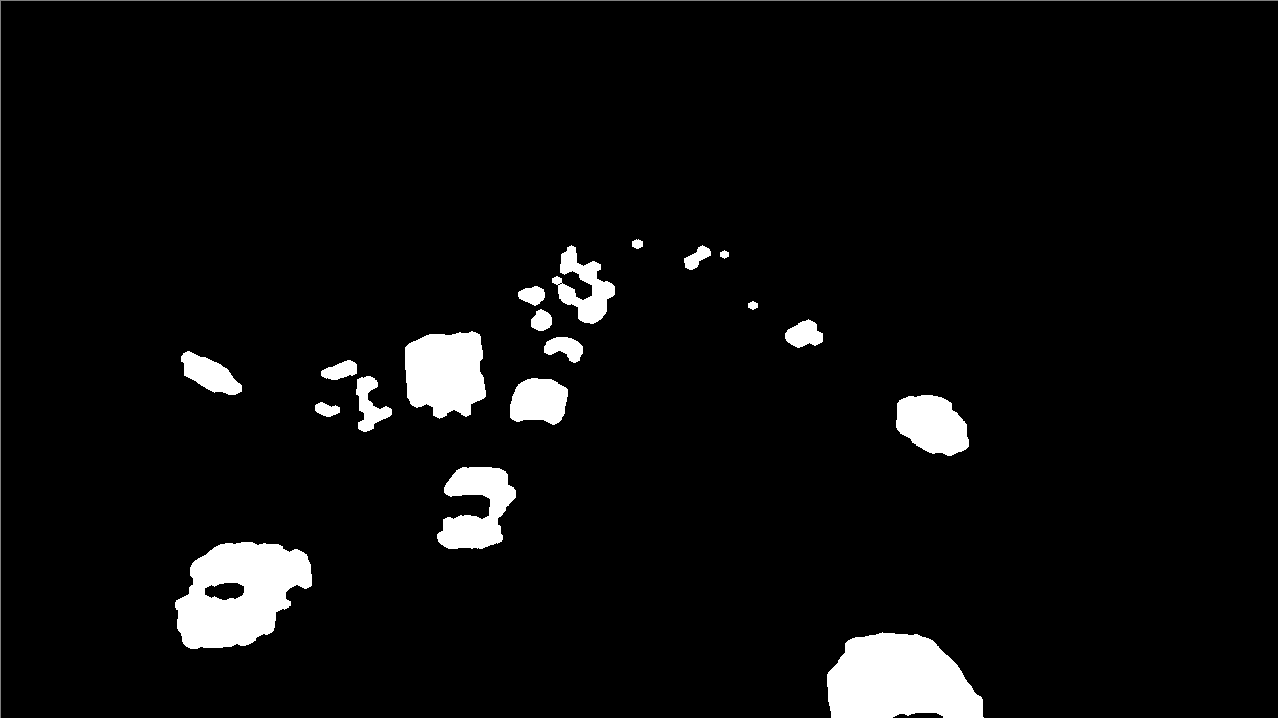
\includegraphics[width=\textwidth]{design/detection/morphology/ellipse_5}
            % \captionsetup{format = hang}
        \end{subfigure} &
        \begin{subfigure}[b]{0.3\textwidth}
            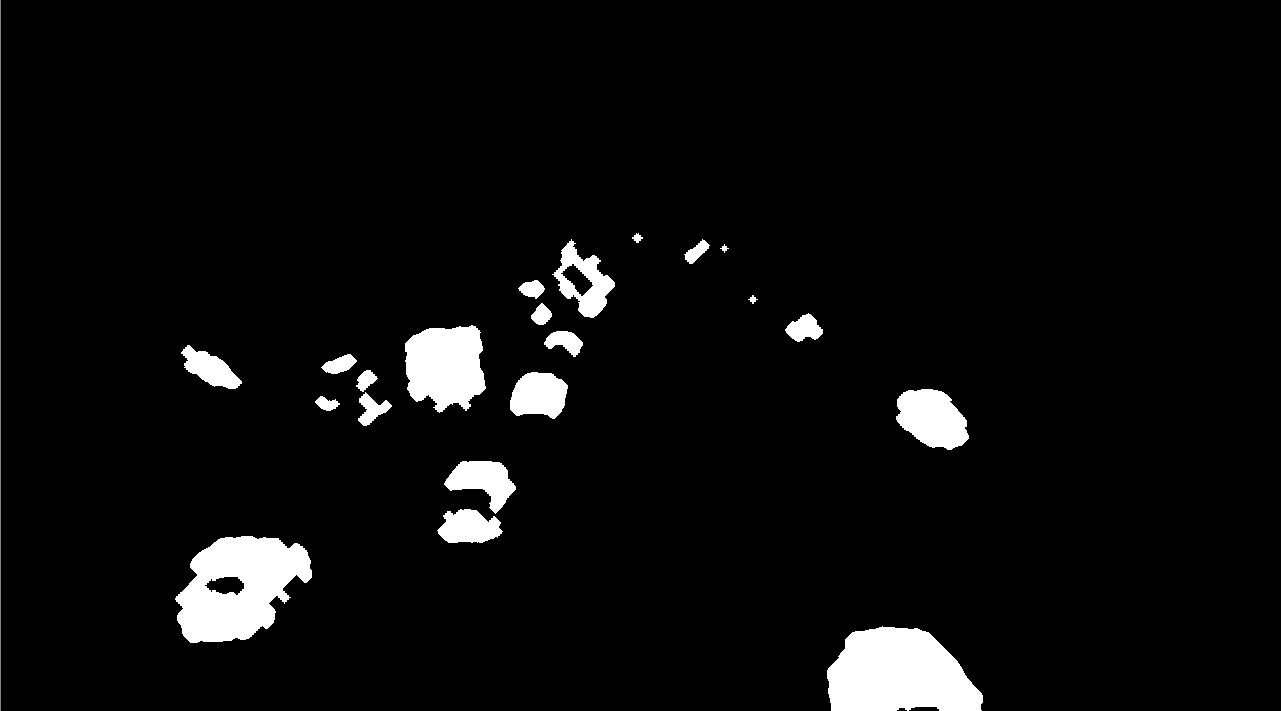
\includegraphics[width=\textwidth]{design/detection/morphology/cross_5}
            % \captionsetup{format = hang}
        \end{subfigure} &
        \begin{subfigure}[b]{0.3\textwidth}
            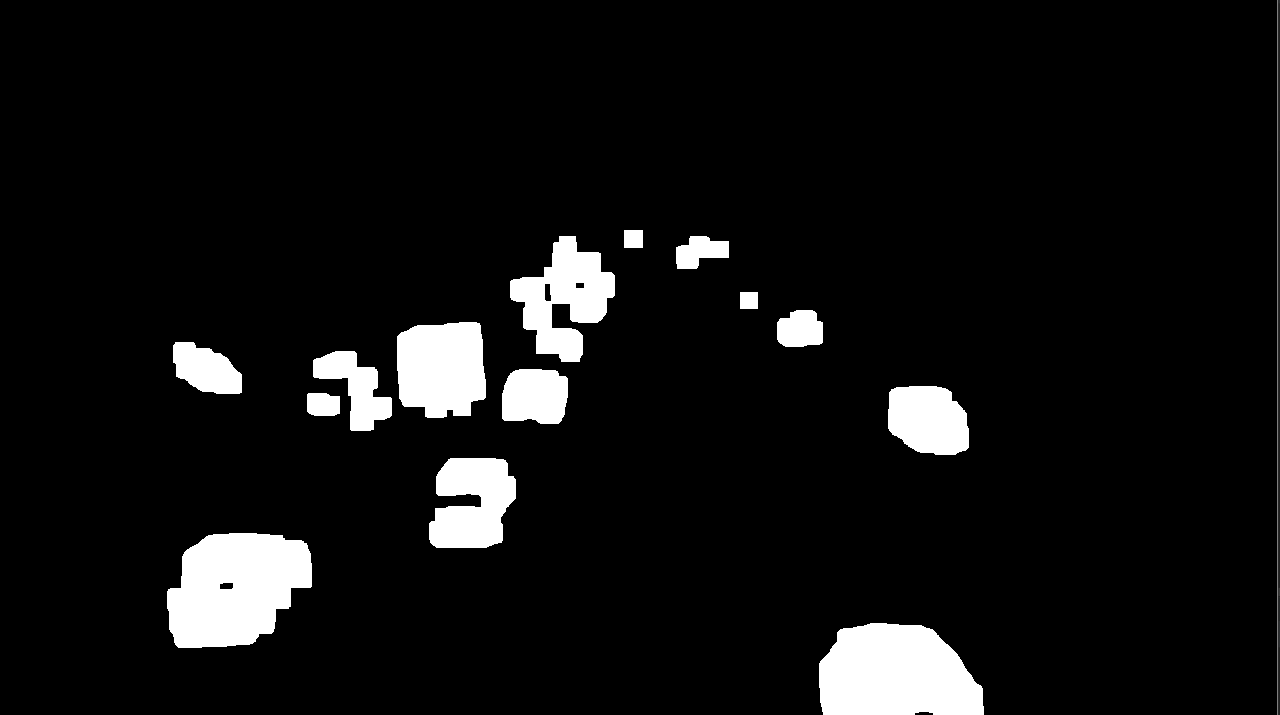
\includegraphics[width=\textwidth]{design/detection/morphology/rect_5}
            % \captionsetup{format = hang}
        \end{subfigure} \\
    \end{tabular}
    \captionsetup{format = hang}
    \caption{Morphological closing using different 7x7 structuring elements and iterations.}
    \label{fig:morph_testing}
\end{figure*}